% ============================================================================
% Informe de Estudio de Conexion Simplificado - CREG 174 de 2021
% Proyecto: Generacion Distribuida 990 kW - Puerto Boyaca (EBSA), circuito 15344
% Listo para pegar en Overleaf. Compilador recomendado: pdfLaTeX.
% ============================================================================
\documentclass[11pt,a4paper]{article}

% --- Idioma y codificacion ---
\usepackage[spanish,es-tabla]{babel}
\usepackage[utf8]{inputenc}
\usepackage[T1]{fontenc}
\usepackage{textcomp} % necesario para \textdegree

% --- Layout y tipografia ---
\usepackage[a4paper,margin=2.5cm]{geometry}
\usepackage{fancyhdr}
\usepackage{titlesec}
\usepackage{setspace}
\onehalfspacing

% --- Tablas, figuras, unidades ---
\usepackage{booktabs}
\usepackage{longtable}
\usepackage{array}
\usepackage{tabularx}
\usepackage{graphicx}
\usepackage{caption}
\usepackage{float}
\usepackage{siunitx}
\sisetup{output-decimal-marker={,}, group-separator={.}}

% --- Listas, colores, enlaces, notas pendientes ---
\usepackage{enumitem}
\usepackage[dvipsnames]{xcolor}
\usepackage[colorlinks=true,linkcolor=NavyBlue,citecolor=NavyBlue,urlcolor=NavyBlue]{hyperref}
\usepackage{todonotes}

% --- Encabezado / pie de pagina ---
\pagestyle{fancy}
\fancyhf{}
\fancyhead[L]{Estudio de Conexi\'on Simplificado -- GD 990\,kW Puerto Boyac\'a}
\fancyhead[R]{\thepage}
\fancyfoot[C]{\small Confidencial -- Uso exclusivo tr\'amite de conexi\'on ante EBSA}
\renewcommand{\headrulewidth}{0.4pt}

% --- Estilo de secciones ---
\titleformat{\section}{\normalfont\Large\bfseries}{\thesection.}{0.6em}{}
\titleformat{\subsection}{\normalfont\large\bfseries}{\thesubsection}{0.6em}{}

% --- Comando corto para marcar contenido pendiente (visible como nota al margen) ---
% Nota: el argumento de \todo se deja corto (solo la etiqueta) a proposito,
% para no arriesgar el limite de \todo con contenido largo/multi-parrafo;
% el texto completo va inline en el cuerpo via \textcolor.
\long\newcommand{\pendiente}[1]{\todo[color=red!40,size=\small]{PENDIENTE}\textcolor{red!70!black}{\textbf{[PENDIENTE: #1]}}}
\long\newcommand{\parcial}[1]{\todo[color=yellow!60,size=\small]{PARCIAL}\textcolor{orange!80!black}{\textbf{[PARCIAL: #1]}}}

\title{\textbf{Informe de Estudio de Conexi\'on Simplificado}\\[0.3em]
\large Generaci\'on Distribuida (GD) -- 990\,kW\\
Circuito 15344, Subestaci\'on Puerto Boyac\'a -- EBSA\\[0.3em]
\normalsize Elaborado en el marco de la Resoluci\'on CREG 174 de 2021}
\author{Interesado en conectarse: Brayan Enrique Aguirre \'Angulo}
\date{Solicitud N\textdegree\ 16869 \\ \today}

\begin{document}

\begin{titlepage}
\maketitle
\thispagestyle{empty}

\vspace{2cm}
\begin{center}
\begin{tabular}{|>{\bfseries}p{5cm}|p{9cm}|}
\hline
Proyecto & Sistema de Generaci\'on Distribuida solar fotovoltaica, 990\,kW \\ \hline
Operador de Red (OR) & Empresa de Energ\'ia de Boyac\'a S.A. E.S.P. (EBSA) \\ \hline
Circuito / Subestaci\'on & 15344 / Puerto Boyac\'a \\ \hline
Nivel de tensi\'on de conexi\'on & Nivel II (13.2\,kV) -- ruta ``Solicitudes N2'' seg\'un Anexo I CREG 174 \\ \hline
Ubicaci\'on & Puerto Boyac\'a, Boyac\'a -- Lat.\ 5.962244, Long.\ $-74.565052$ \\ \hline
A\~no de entrada en operaci\'on (a\~no $t$) & \textbf{2026} \\ \hline
A\~no de an\'alisis posterior ($t+x$) & \pendiente{solicitar valor de $x$ vigente al OR} \\ \hline
\end{tabular}
\end{center}

\vspace{1.5cm}
\begin{center}
\begin{tabular}{|c|c|p{8cm}|}
\hline
\textbf{Revisi\'on} & \textbf{Fecha} & \textbf{Descripci\'on} \\ \hline
0 & \today & Primera estructura del informe, a partir de insumos ya montados en PowerFactory \\ \hline
& & \\ \hline
\end{tabular}
\end{center}
\end{titlepage}

\tableofcontents
\listoftodos[Pendientes del informe]
\clearpage

% ============================================================================
\section{Resumen ejecutivo}
% CREG 174, numeral 6.1
\pendiente{Redactar al final, cuando estén cerrados los resultados de las secciones 5 y 6.}

\subsection*{Antecedentes y alcance del proyecto}
\pendiente{Antecedentes de la solicitud, alcance del estudio.}

\subsection*{Supuestos principales}
\pendiente{Resumir supuestos clave (herramienta de simulación: DIgSILENT PowerFactory 2024; método de cortocircuito: IEC 60909 / VDE 0102 Part 0; automatización de los cálculos vía scripts Python descritos en este documento).}

\subsection*{Resumen de resultados}
\pendiente{Completar cuando estén los resultados finales de flujo de carga y cortocircuito para los escenarios 8.2.2 y 8.2.3.}

\subsection*{Conclusiones}
\pendiente{Ver Secci\'on \ref{sec:conclusiones}.}

% ============================================================================
\section{Descripci\'on y ubicaci\'on del proyecto}
% CREG 174, numeral 6.2
\parcial{Falta texto descriptivo (antecedentes) y figura de ubicaci\'on geogr\'afica.}

\subsection*{Descripci\'on general}
\begin{itemize}
    \item \textbf{Tipo de fuente de energ\'ia:} Solar fotovoltaica on-grid, 1456 paneles Trina Solar TSM-NEG21C.20 (720\,Wp, bifacial N-type i-TOPCon) + 3 inversores Huawei SUN2000-330KTL-H1 (330\,kW c/u).
    \item \textbf{Capacidad:} 1048.36\,kWp DC nominal (STC) / 1190.89\,kWp DC real con ganancia por bifacialidad / \textbf{990\,kW AC} (factor de potencia unitario). Fuente: Memoria de c\'alculo, Tabla 14 ``Resumen T\'ecnico del Sistema''.
    \item \textbf{Vida \'util:} \textbf{30 a\~nos} (confirmado con el interesado; coincide con la garant\'ia de potencia del panel Trina Solar, 87.4\,\% a 30 a\~nos).
    \item \textbf{Punto de conexi\'on:} Barra ``Puerto Boyaca 800V'', circuito 15344, a trav\'es de transformador de elevaci\'on 1250\,kVA (Z=8\,\%), 800\,V AC / 13.2\,kV.
\end{itemize}

\textbf{Correcci\'on (2026-09-18):} en una corrida anterior de \texttt{Flujo\_carga.py} el generador aparec\'ia despachando ``990'' en un campo que se interpret\'o -- err\'oneamente -- como MW en vez de kW, lo que suger\'ia un problema en la configuraci\'on del modelo. \textbf{El modelo estaba correcto desde el principio.} El error era del script: los resultados de flujo de carga (\texttt{ComLdf}) en este proyecto de PowerFactory vienen nativamente en kW/kvar/A, no en MW/Mvar/kA como se hab\'ia asumido. Verificado cruzando generadores, l\'ineas y el transformador propio contra c\'alculos f\'isicos esperados -- todos cuadran exactamente al reinterpretar esos valores como kW/A. Corregido en \texttt{Flujo\_carga.py} (divisi\'on entre 1000 aplicada a las variables de flujo de carga; las variables de cortocircuito de \texttt{Cortocircuito.py} no necesitaban correcci\'on, ya val\'ian en kA nativamente).

\subsection*{Ubicaci\'on geogr\'afica}
Se reportan dos coordenadas, correspondientes a dos puntos distintos del proyecto (confirmado con el interesado):
\begin{itemize}
    \item \textbf{Punto de conexi\'on a la red EBSA} (ficha de insumos, solicitud 16869): Latitud 5.962244, Longitud $-74.565052$.
    \item \textbf{Ubicaci\'on f\'isica de la planta} (paneles/inversores, seg\'un memoria de c\'alculo): Latitud 5.963004, Longitud $-74.5664488$, altura 130\,msnm.
\end{itemize}
\pendiente{Insertar imagen satelital/mapa de ubicaci\'on (idealmente mostrando ambos puntos: conexi\'on y planta).}

\subsection*{Diagrama unifilar general}
\pendiente{Insertar el diagrama unifilar exportado por \texttt{Flujo\_carga.py} / \texttt{Cortocircuito.py} (carpeta \texttt{resultados/graficos\_red/} o \texttt{graficos\_red\_corto/}). Los diagramas se exportan en formato SVG; para incluirlos en pdfLaTeX conv\'ertalos primero a PDF (por ejemplo con Inkscape: \texttt{inkscape archivo.svg --export-type=pdf}) y use:}
\begin{verbatim}
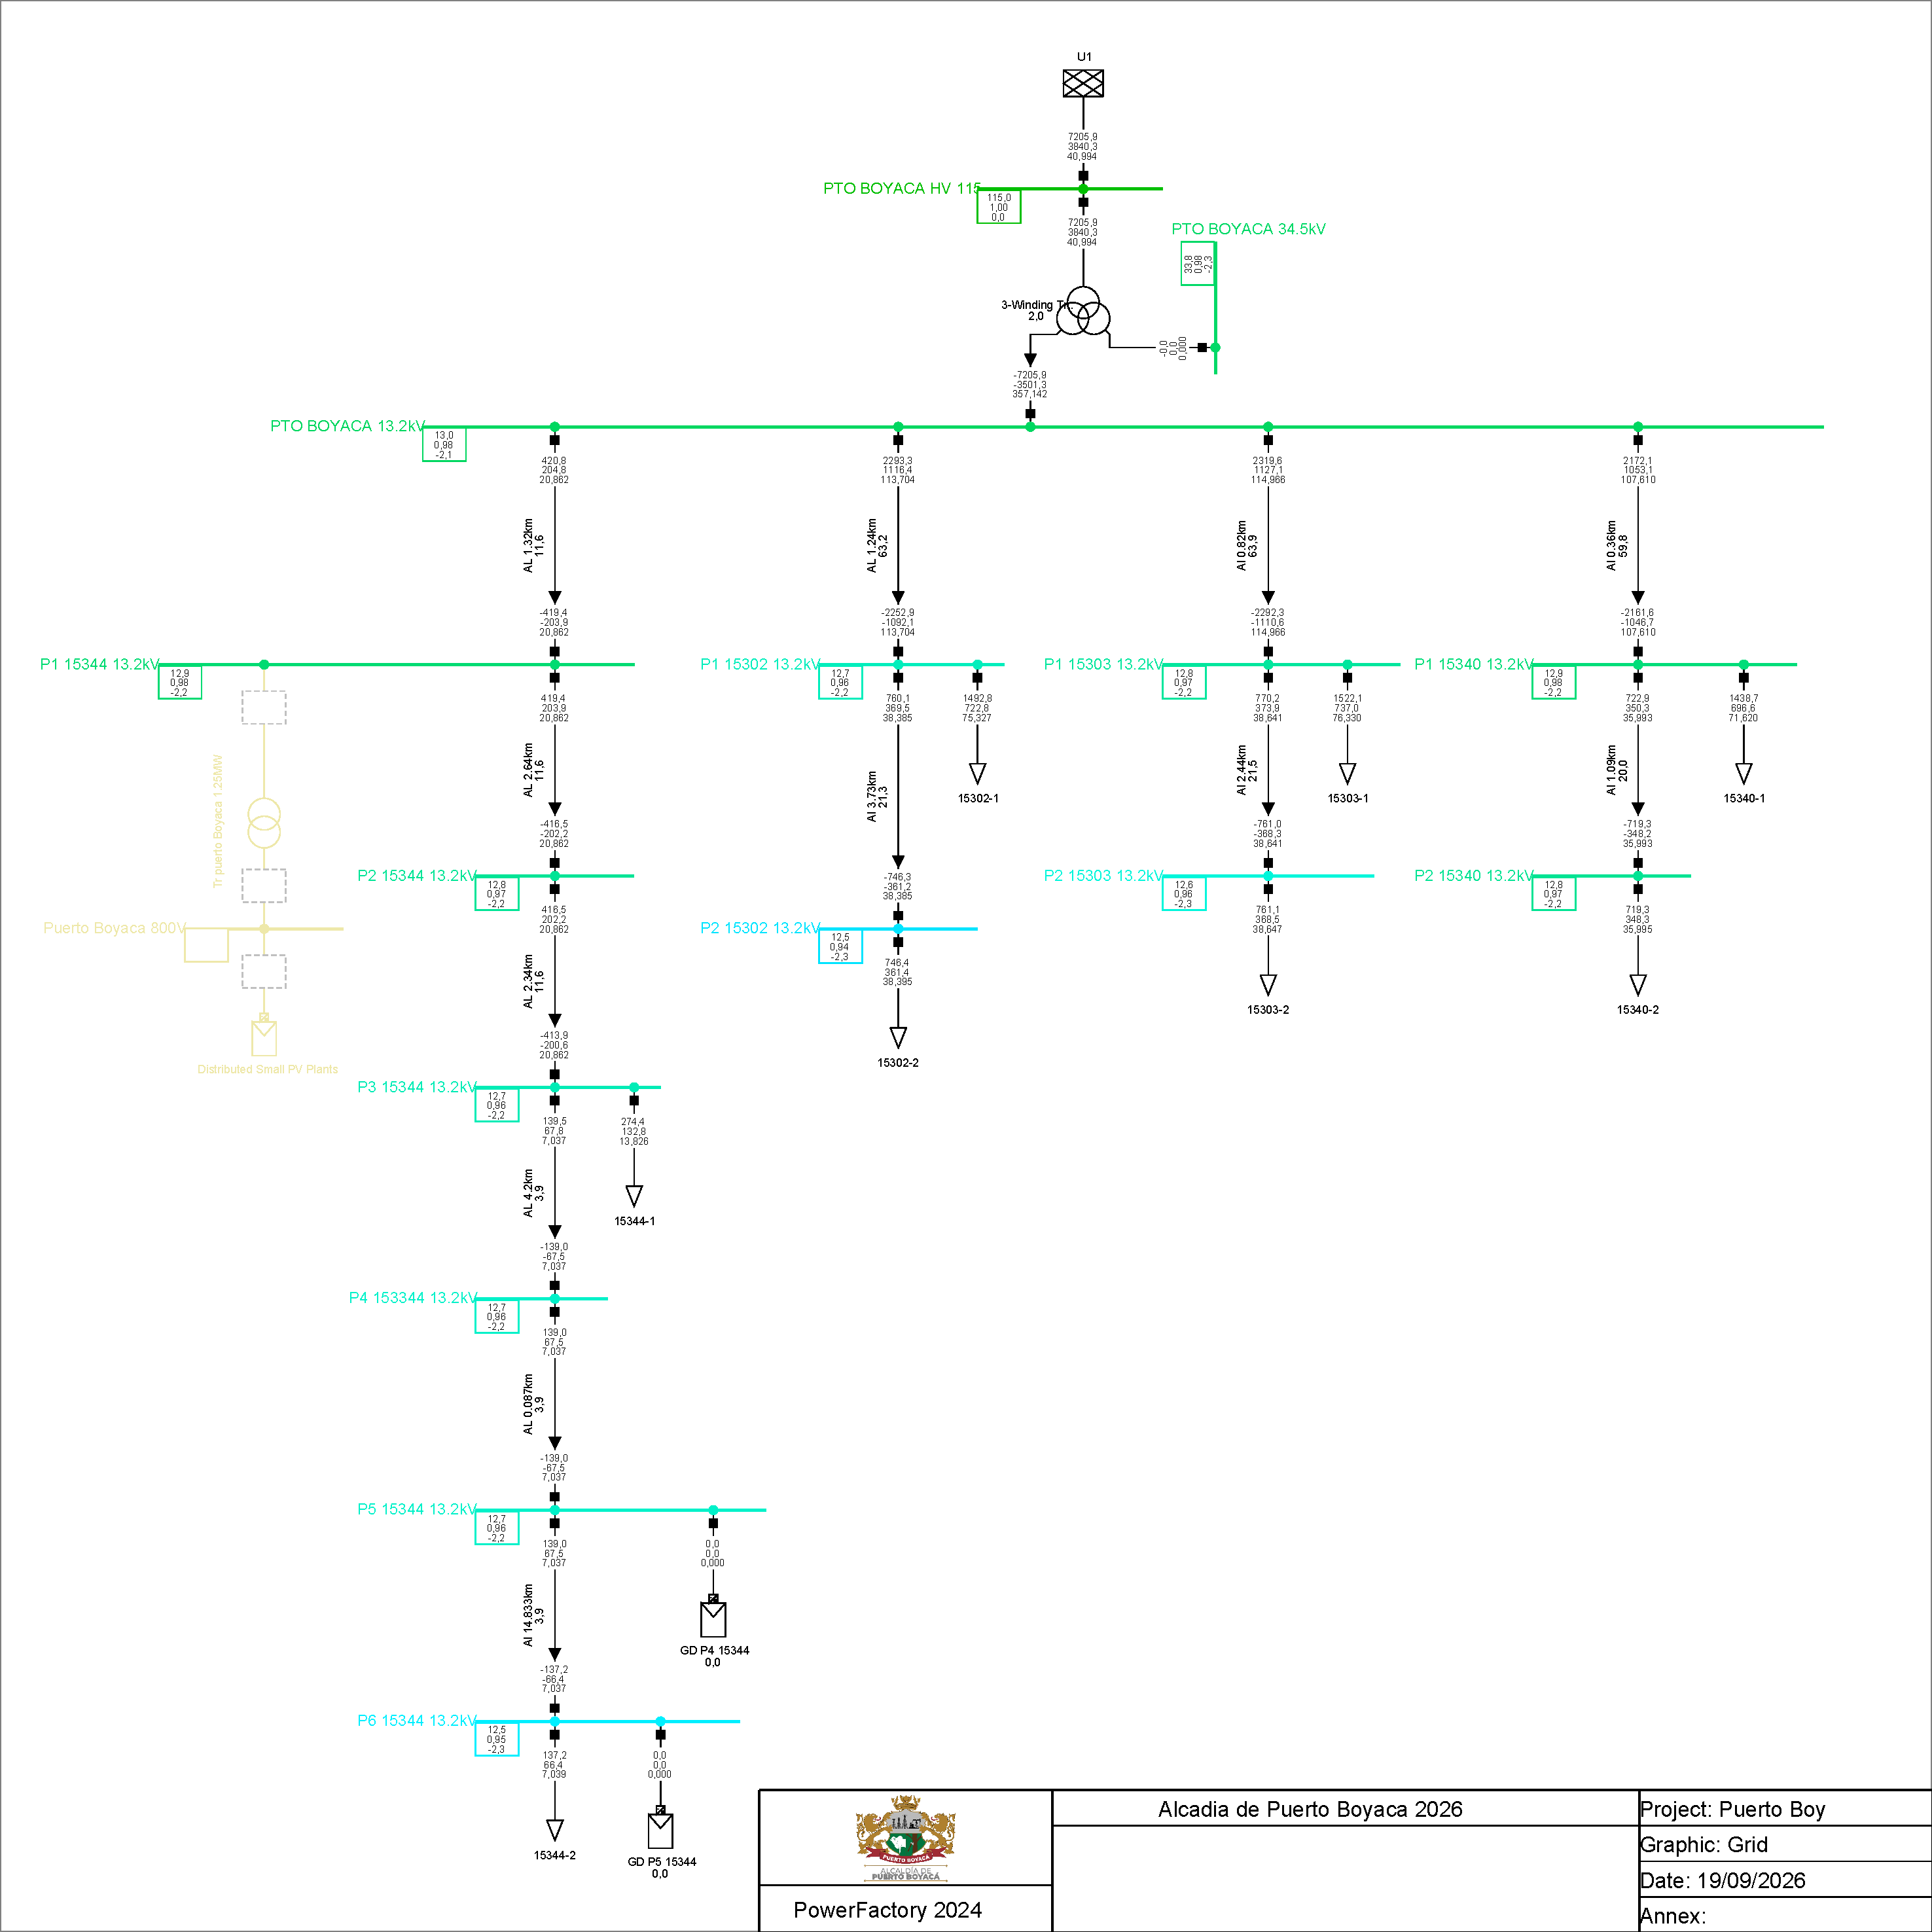
\includegraphics[width=\textwidth]{diagrama_unifilar.pdf}
\end{verbatim}

% ============================================================================
\section{Par\'ametros el\'ectricos de los equipos del proyecto}
\label{sec:parametros}
% CREG 174, numeral 6.3, Tablas 1 a 5

\subsection{Transformadores (Tabla 1)}
\begin{table}[H]
\centering
\caption{Datos del transformador T9 (subestaci\'on Puerto Boyac\'a)}
\begin{tabular}{lccccccc}
\toprule
Nombre & Devanados & HV (kV) & MV (kV) & LV (kV) & $S_{HV}$ (MVA) & $S_{MV}$ (MVA) & $S_{LV}$ (MVA) \\
\midrule
T9 & 3 & 115 & 34.5 & 13.8 & 20 & 20 & 20 \\
\bottomrule
\end{tabular}

\vspace{0.5em}
\begin{tabular}{lccc}
\toprule
Grupo de conexi\'on & $u_{k,HV-MV}$ (\%) & $u_{k,HV-LV}$ (\%) & $u_{k,MV-LV}$ (\%) \\
\midrule
YNyn0yn0(d1) & 17.43 & 10.17 & 5.6 \\
\bottomrule
\end{tabular}
\vspace{0.3em}

\small Notas: posici\'on neutra de TAP = 7, m\'axima = 1, m\'inima = 15. Sobrecarga en emergencia 120\,\%.
\end{table}

\pendiente{Transformador propio del proyecto (``Tr puerto Boyaca 1.25MW''): agregar capacidad, grupo de conexi\'on, impedancias y datos de TAP si aplica.}

\subsection{L\'ineas de conexi\'on y cableado principal (Tabla 2)}
\begin{table}[H]
\centering
\caption{Tramos del circuito troncal 15344}
\begin{tabular}{llcccc}
\toprule
Desde & Hasta & Long.\ (km) & Conductor & $R$ ($\Omega$/km) & $X$ ($\Omega$/km) \\
\midrule
PTO BOYACA LV & P1\_15344 & 1.32 & AL Sparrow \#2 (2 ACSR) & 0.8409 & 0.5056 \\
P1\_15344 & P2\_15344 & 2.64 & AL Sparrow \#2 (2 ACSR) & 0.8409 & 0.5056 \\
P2\_15344 & P3\_15344 & 2.34 & AL Sparrow \#2 (2 ACSR) & 0.8409 & 0.5056 \\
P3\_15344 & P4\_15344 & 4.20 & AL Sparrow \#2 (2 ACSR) & 0.8409 & 0.5056 \\
P4\_15344 & P5\_15344 & 0.087 & AL Sparrow \#2 (2 ACSR) & 0.8409 & 0.5056 \\
P5\_15344 & P6\_15344 & 14.833 & AL Sparrow \#2 (2 ACSR) & 0.8409 & 0.5056 \\
\bottomrule
\end{tabular}
\end{table}

\subsection{Datos de placa del generador (Tablas 3 y 4)}
Fuente: fichas t\'ecnicas del fabricante (\texttt{informe/Panel solar/}, \texttt{informe/Inversor/}) y memoria de c\'alculo del proyecto.

\begin{table}[H]
\centering
\caption{Resumen del sistema fotovoltaico}
\begin{tabular}{ll}
\toprule
Par\'ametro & Valor \\
\midrule
Cantidad de inversores & 3 \\
Paneles totales en planta & 1456 \\
Potencia DC nominal (STC) & 1048.36\,kWp \\
Potencia DC real (con bifacialidad) & 1190.89\,kWp \\
Potencia AC nominal & 990\,kW \\
Factor de potencia nominal & 1.0 \\
Tensi\'on de conexi\'on (salida inversores) & 800\,V AC \\
\bottomrule
\end{tabular}
\end{table}

\begin{table}[H]
\centering
\caption{Datos de placa -- Panel solar Trina Solar TSM-NEG21C.20 (720\,Wp)}
\begin{tabular}{ll}
\toprule
Par\'ametro & Valor \\
\midrule
Tecnolog\'ia & N-type i-TOPCon bifacial, doble vidrio, monocristalino \\
Potencia m\'axima $P_{MAX}$ (STC) & 720\,W \\
Eficiencia m\'axima & 23.2\,\% \\
Tensi\'on en punto de m\'axima potencia $V_{MPP}$ & 41.3\,V \\
Corriente en punto de m\'axima potencia $I_{MPP}$ & 17.44\,A \\
Tensi\'on de circuito abierto $V_{OC}$ & 49.4\,V \\
Corriente de cortocircuito $I_{SC}$ & 18.49\,A \\
Coeficiente de temperatura de $P_{MAX}$ & $-0.29\,\%/^{\circ}$C \\
Coeficiente de temperatura de $V_{OC}$ & $-0.24\,\%/^{\circ}$C \\
Coeficiente de temperatura de $I_{SC}$ & $+0.04\,\%/^{\circ}$C \\
Tensi\'on m\'axima de sistema & 1500\,V DC \\
N\'umero de celdas & 132 \\
Bifacialidad & $80\pm5\,\%$ \\
Garant\'ia de potencia & 87.4\,\% a 30 a\~nos \\
\bottomrule
\end{tabular}
\end{table}

\begin{table}[H]
\centering
\caption{Datos de placa -- Inversor Huawei SUN2000-330KTL-H1}
\begin{tabular}{ll}
\toprule
Par\'ametro & Valor \\
\midrule
Topolog\'ia & Sin transformador (transformerless) \\
Potencia activa nominal AC & 300\,kW \\
Potencia aparente m\'axima AC & 330\,kVA \\
Tensi\'on nominal de salida & 800\,V, 3W + PE \\
Corriente nominal de salida & 216.6\,A \\
Corriente m\'axima de salida & 238.2\,A \\
N\'umero de MPPT & 6 \\
Corriente m\'axima por MPPT & 65\,A \\
Corriente m\'axima de cortocircuito por MPPT & 115\,A \\
Rango de tensi\'on MPPT & 500\,--\,1500\,V DC \\
Tensi\'on nominal de entrada & 1080\,V DC \\
Rango de factor de potencia ajustable & 0.8 en adelanto -- 0.8 en atraso \\
Distorsi\'on arm\'onica total (THDi) & $<1\,\%$ a potencia nominal (l\'imite normativo: 5\,\%) \\
Protecci\'on anti-isla & Certificado IEC 62116 / IEEE 1547 / UL 1741 \\
\bottomrule
\end{tabular}
\end{table}
\parcial{Aporte de los inversores a la corriente de cortocircuito: seg\'un la memoria de c\'alculo, limitado a $\approx 1.1\times I_n$ por la electr\'onica de potencia (no aportan corriente de falla significativa, comportamiento t\'ipico de generaci\'on basada en inversores). \textbf{Esto explica} el resultado de \texttt{Cortocircuito.py} donde el generador mostraba $I_{kss}=0$ en todas las fallas -- el objeto \texttt{ElmPvsys} en PowerFactory probablemente no tiene configurado su aporte a cortocircuito (deber\'ia ser $\approx 1.1\times 216.6\,A \approx 0.24$\,kA por inversor, no cero). Pendiente corregir en el modelo (pesta\~na Short-Circuit VDE/IEC del objeto).}

\subsection{Elementos adicionales (Tabla 5)}
El proyecto \textbf{no cuenta} con control central de planta (PPC) ni con compensaci\'on reactiva adicional (bancos de condensadores o reactores) -- confirmado con el interesado. En su lugar, el propio inversor Huawei SUN2000-330KTL-H1 cumple la funci\'on de control de tensi\'on en el punto de conexi\'on, mediante su capacidad de potencia reactiva ajustable (rango de factor de potencia 0.8 en adelanto -- 0.8 en atraso, ver Secci\'on~\ref{sec:parametros}), seg\'un sea necesario y conforme a la regulaci\'on t\'ecnica aplicable.

% ============================================================================
\section{Informaci\'on de entrada y supuestos para el an\'alisis}
% CREG 174, numeral 6.4 / numeral 7

\subsection{Modelaci\'on de la zona de influencia}
% 7.1.2 - Nivel de tension N2
Solicitud de conexi\'on al Nivel de Tensi\'on II (7.1.2 de CREG 174). Informaci\'on suministrada/asumida:
\begin{itemize}
    \item \textbf{Equivalente de la subestaci\'on:} $I_{cc,3F} = 6.002$\,kA, $I_{cc,1F} = 2.622$\,kA, $X/R = 10$ (barra 115\,kV).
    \item \textbf{Red troncal principal:} circuito 15344, tramos P1 a P6 (conductor \'unico AL Sparrow \#2), ver Tabla en Secci\'on~\ref{sec:parametros}.
    \item \textbf{Demanda equivalente:} curva horaria de 8 cargas del \'area de influencia (15302-1/2, 15303-1/2, 15340-1/2, 15344-1/2), horas 6 a 17 -- ver \texttt{inputs/Parametros\_Demanda.xlsx}.
    \item \textbf{Generadores conectados al circuito:} planta solar objeto de este estudio (990\,kW), \textbf{m\'as dos generadores distribuidos ya existentes} en el circuito 15344 seg\'un EBSA (\texttt{DOC\_REF\_EST\_1787069892338.pdf}, ``Generadores Distribuidos Conectados: 2''): \textbf{GD1} (330\,kVA, barra P4\_15344) y \textbf{GD2} (330\,kVA, barra P5\_15344). CREG 174 (num.\ 8.4) exige considerar ``toda la generaci\'on de la zona en l\'inea'' -- estos dos generadores no estaban modelados previamente; se agregan \textbf{manualmente} a la red base en PowerFactory (no como Network Variation, porque ya existen con independencia del proyecto nuevo).

    \textbf{Supuestos gen\'ericos adoptados para GD1/GD2} (no se tiene ni se puede tener la ficha t\'ecnica real -- son equipos de un tercero, no del interesado en este estudio):
    \begin{itemize}
        \item Factor de potencia unitario ($\cos\varphi=1$), consistente con el dato de EBSA.
        \item Despacho: mismo criterio de generaci\'on no gestionable que el proyecto propio (0\,MW en el escenario de carga pura; en las dem\'as horas, mismo perfil de Horas Pico Solar de la zona, Secci\'on~\ref{sec:parametros}, escalado a 330\,kVA).
        \item \textbf{Aporte a cortocircuito: ``No Short-Circuit Contribution'' (aporte cero)}. Decisi\'on justificada, no arbitraria: (i) es el tratamiento por defecto de PowerFactory ante un generador sin datos de fabricante; (ii) es f\'isicamente razonable para generaci\'on tipo inversor, que ya vimos que aporta poco incluso con datos reales ($\approx$1.1$\times I_n$ en el proyecto propio); y (iii) es la asunci\'on que \textbf{menos consume} la capacidad de corte disponible (10\,kA) para evaluar el proyecto propio -- la m\'as favorable para su viabilidad, sin fabricar datos que no se tienen.
    \end{itemize}

    \pendiente{Una vez montados GD1/GD2 en PowerFactory (manualmente) y recalculados \texttt{Flujo\_carga.py}/\texttt{Cortocircuito.py}, comparar cargabilidad/tensi\'on en el tramo P2-P3 y en T9, y el margen de Icc en P3/800\,V respecto a 10\,kA, \textbf{antes vs.\ despu\'es} de incluir GD1/GD2 -- esto cuantifica cu\'anto limitan estos dos generadores existentes la capacidad disponible en el punto de conexi\'on del proyecto propio. Todos los resultados de flujo de carga y cortocircuito de este informe deben recalcularse incluyendo GD1/GD2 en el \texttt{CasoBase}.}
    \item \textbf{Condiciones operativas principales} (ajustes de protecci\'on de la cabecera del circuito, tomados del documento de insumos de EBSA): curva IEC Normal Inverse, Pickup 51 = 240\,A, Pickup 51N = 60\,A, Dial 51 = 0.1, Dial 51N = 0.1, instant\'aneo de fase (50) = 1500\,A, instant\'aneo de tierra (50N) = 300\,A, tiempo de recierre r\'apido del reconectador = 2\,s. Transformador T9: TAP neutro = 7, m\'aximo = 1, m\'inimo = 15; sobrecarga en emergencia = 120\,\%, tiempo de emergencia = 30\,min.
    \item \textbf{Capacidad de cortocircuito (interrupci\'on) de la subestaci\'on:} \textbf{10\,kA} (documento de insumos EBSA). Este es el valor a contrastar contra los resultados de la Secci\'on~\ref{sec:cortocircuito}. Como referencia adicional (no oficial del OR), la memoria de c\'alculo del proyecto reporta, para el transformador de elevaci\'on propio 1250\,kVA / Z=8\,\%: $I_{cc,3F}=11.2$\,kA en el lado de 800\,V, e $I_{f}=2.799$\,kA (falla a tierra) en el lado de 13.2\,kV.
\end{itemize}

\subsection{Horizonte de an\'alisis}
\label{sec:parametros-t}
A\~no $t = \mathbf{2026}$ (entrada en operaci\'on, confirmado con el interesado). A\~no $t+x = \mathbf{2028}$ ($x=2$, seg\'un el documento de insumos de EBSA para esta solicitud -- el OR indica expl\'icitamente ``el a\~no dos (2) posterior a la puesta en servicio del proyecto''). Para el escenario del a\~no $t+x$, EBSA solicita considerar un \textbf{incremento del 1.04\,\% en la demanda}.

\subsection{Informaci\'on de demanda de potencia}
Curvas de demanda horaria (horas 6 a 17) para las 8 cargas del \'area de influencia del circuito 15344, transcritas de la tabla ``CARGA PTO BOYAC\'A 34,5kV'' suministrada por EBSA y verificadas valor por valor contra la fuente. Ver \texttt{inputs/Parametros\_Demanda.xlsx}.

\subsection{Informaci\'on de compensaci\'on reactiva en el \'area}
\pendiente{No se encontr\'o menci\'on de bancos de condensadores/reactores del OR en la documentaci\'on revisada -- solicitar al OR si existen en la zona de influencia.}

\subsection{Informaci\'on de la energ\'ia producida}
Seg\'un la memoria de c\'alculo, con Horas Pico Solar (HPS) promedio de 4.152\,kWh-d\'ia y $PR=0.85$, la generaci\'on mensual promedio proyectada es de \textbf{110\,998.61\,kWh} (Tabla 15). A partir de la irradiaci\'on mensual real reportada en la memoria (Tabla 3, plataforma Atlas Global Solar) se calcula el desglose mes a mes para el a\~no 1 (2026), y la proyecci\'on anual para el resto de la vida \'util (30 a\~nos) aplicando la curva de degradaci\'on del fabricante del panel (1\,\% el primer a\~no, 0.4\,\%/a\~no despu\'es -- ficha t\'ecnica Trina Solar).

\begin{table}[H]
\centering
\caption{Generaci\'on mensual estimada -- A\~no 1 (2026)}
\begin{tabular}{lcc}
\toprule
Mes & HPS (kWh/m$^2$-d\'ia) & Generaci\'on estimada (kWh) \\
\midrule
Enero & 4.340 & 119\,891.93 \\
Febrero & 3.738 & 93\,268.68 \\
Marzo & 3.156 & 87\,184.08 \\
Abril & 3.521 & 94\,129.51 \\
Mayo & 4.056 & 112\,046.46 \\
Junio & 4.484 & 119\,874.10 \\
Julio & 4.913 & 135\,720.97 \\
Agosto & 4.637 & 128\,096.51 \\
Septiembre & 4.411 & 117\,922.54 \\
Octubre & 4.070 & 112\,433.21 \\
Noviembre & 4.164 & 111\,319.30 \\
Diciembre & 4.337 & 119\,809.05 \\
\midrule
\textbf{Total a\~no 1} & -- & \textbf{1\,351\,696.35} \\
\bottomrule
\end{tabular}
\end{table}

\begin{table}[H]
\centering
\caption{Generaci\'on anual estimada -- a\~nos 2 a 30 (con degradaci\'on del panel)}
\begin{tabular}{cccccccc}
\toprule
A\~no & 2 & 3 & 10 & 15 & 20 & 25 & 30 \\
\midrule
Factor & 99.0\,\% & 98.6\,\% & 95.8\,\% & 93.8\,\% & 91.8\,\% & 89.8\,\% & 87.8\,\% \\
Generaci\'on (kWh) & 1\,338\,179 & 1\,332\,773 & 1\,294\,925 & 1\,267\,891 & 1\,240\,857 & 1\,213\,823 & 1\,186\,789 \\
\bottomrule
\end{tabular}
\end{table}
\parcial{C\'alculo propio (no viene as\'i en la memoria original), a partir de datos que s\'i est\'an en la memoria (irradiaci\'on mensual Tabla 3, degradaci\'on del panel). Verificar que el criterio de degradaci\'on lineal 1\,\%/0.4\,\% sea aceptable o si se prefiere usar directamente el 87.4\,\% garantizado a 30 a\~nos como \'unico punto de referencia.}

Adicionalmente, la memoria de c\'alculo incluye un perfil de generaci\'on m\'axima hora a hora (Tabla 16, datos de Atlas Global Solar), que se reutiliza en la Secci\'on~\ref{sec:escenarios} para identificar los escenarios de estudio:
\begin{table}[H]
\centering
\caption{Generaci\'on solar m\'axima por hora (memoria de c\'alculo, Tabla 16)}
\begin{tabular}{cc}
\toprule
Hora & Generaci\'on m\'axima (kWh) \\
\midrule
6--7 & 89.11 \\
7--8 & 218.31 \\
8--9 & 328.81 \\
9--10 & 427.71 \\
10--11 & 507.91 \\
\textbf{11--12} & \textbf{564.05 (m\'aximo)} \\
12--13 & 556.92 \\
13--14 & 521.28 \\
14--15 & 453.56 \\
15--16 & 390.29 \\
16--17 & 285.14 \\
17--18 & 118.51 \\
\bottomrule
\end{tabular}
\end{table}

% ============================================================================
\section{Presentaci\'on de an\'alisis}
% CREG 174, numeral 6.5 / numeral 8

\subsection{Validaci\'on de la correcta modelaci\'on}
\label{sec:validacion}
% 8.1
Topolog\'ia, nivel de cortocircuito y perfil de tensiones/cargabilidad del sistema \textbf{sin} el proyecto de generaci\'on (escenario de carga pura, taps fijos en posici\'on central, nodo slack en el equivalente de red). Topolog\'ia radial (SE Puerto Boyac\'a $\to$ P1 $\to$ P2 $\to$ \ldots $\to$ P6), sin caminos alternos -- ver diagrama unifilar (Secci\'on~\ref{sec:parametros} y anexos del documento de insumos EBSA).

\textbf{Limitaci\'on identificada respecto al m\'etodo que exige CREG 174:} el numeral 8.1 asume que el OR entrega sus propios resultados de tensi\'on/cargabilidad/cortocircuito para comparar contra los del interesado (causal de rechazo si la desviaci\'on supera el 10\,\%, numeral 10.1). En este caso, \textbf{EBSA \'unicamente suministr\'o datos de entrada} (equivalente de red, topolog\'ia, par\'ametros del transformador, ajustes de protecci\'on -- documento \texttt{DOC\_REF\_EST\_1787069892338.pdf}), \textbf{no resultados de flujo de carga ni de cortocircuito propios}. Por lo tanto, \textbf{no es posible realizar la comparaci\'on del 10\,\% tal como la plantea el numeral 8.1} -- los resultados presentados en este informe son los \'unicos disponibles, calculados \'integramente por el interesado a partir de los insumos entregados por el OR.

\textbf{An\'alisis alternativo propuesto (con y sin proyecto):} en ausencia de un c\'alculo de referencia del OR, se propone documentar la \textbf{desviaci\'on estad\'istica} de cargabilidad y tensi\'on entre el \texttt{CasoBase} (sin proyecto) y el caso con el generador activo, para las 12 horas simuladas, como evidencia del impacto real del proyecto sobre la red existente:
\pendiente{Calcular, para cada elemento (l\'inea/transformador), el \% de cambio en cargabilidad y tensi\'on entre \texttt{CasoBase} y el caso con GD, y reportar el promedio, m\'aximo y desviaci\'on est\'andar de esa diferencia a lo largo de las 12 horas -- se obtiene directamente de \texttt{Resultados\_Flujo\_Carga\_2026.xlsx} una vez consolidados ambos casos.}

\subsubsection*{Metodolog\'ia detallada de c\'alculo de cortocircuito (para reemplazar el valor simplificado de la memoria de c\'alculo)}
\label{sec:metodologia-corto}
La memoria de c\'alculo del interesado estim\'o $I_{cc,3F}=11.2$\,kA en el lado de 800\,V usando \'unicamente el transformador de elevaci\'on propio (1250\,kVA, $Z=8\,\%$), asumiendo un ``bus infinito'' (impedancia cero) del lado de 13.2\,kV. Esa es una pr\'actica com\'un y \textbf{conservadora} para dimensionar protecciones (nunca subestima la corriente), pero \textbf{no refleja la impedancia real de la red aguas arriba} (equivalente de 115\,kV + transformador T9 + l\'ineas del circuito 15344) que S\'I limita la corriente de falla real. A continuaci\'on se muestra el c\'alculo considerando la red completa, seg\'un el m\'etodo de la fuente de tensi\'on equivalente de IEC 60909 ($I_k'' = \dfrac{c \cdot U_n}{\sqrt{3}\, Z_k}$, con $c=1.1$ para c\'alculo m\'aximo):

\begin{enumerate}
    \item \textbf{Equivalente de red en 115\,kV} ($I_{cc,3F}=6.002$\,kA, $X/R=10$): $Z = \dfrac{1.1 \times 115{,}000}{\sqrt{3}\times 6002} = 12.17\,\Omega$ (R=1.21, X=12.11\,$\Omega$).
    \item \textbf{Transformador T9} (115/13.8\,kV, 20\,MVA, $u_k=10.17\,\%$, referido al lado de 13.8\,kV): $Z_{T9} = 0.1017 \times \dfrac{13{,}800^2}{20\times10^6} = 0.968\,\Omega$.
    \item Referir el equivalente de 115\,kV a la base de 13.8\,kV: $Z_{eq,ref} = 12.17 \times \left(\dfrac{13.8}{115}\right)^2 = 0.175\,\Omega$.
    \item \textbf{L\'ineas del circuito 15344} (SE$\to$P1$\to$P2$\to$P3, conductor \'unico AL Sparrow \#2): $R=5.298\,\Omega$, $X=3.185\,\Omega$, $|Z|=6.18\,\Omega$.
    \item \textbf{Impedancia total en P3 (13.2\,kV)}: $Z_{P3} \approx 0.175+0.968+6.18 = 7.33\,\Omega$ $\Rightarrow$ $I_{k3}'' \approx \dfrac{1.1\times 13{,}200}{\sqrt{3}\times 7.33} \approx \mathbf{1.14\,kA}$.
    \textbf{Verificaci\'on cruzada}: PowerFactory (\texttt{Cortocircuito.py}, \texttt{CasoBase}) calcul\'o $I_{kss}=1.236$\,kA en esa misma barra -- diferencia de $\sim$7\,\%, esperable porque este c\'alculo manual suma magnitudes de impedancia en vez de sumar fasores complejos exactos (PowerFactory s\'i resuelve la matriz de red completa). Confirma que la metodolog\'ia es correcta.
    \item \textbf{Transformador propio del proyecto} (1250\,kVA, $Z=8\,\%$, 800\,V): $Z_{proy} = 0.08\times\dfrac{800^2}{1.25\times10^6} = 0.0410\,\Omega$.
    \item Referir $Z_{P3}$ a la base de 800\,V: $Z_{P3,ref} = 7.33\times\left(\dfrac{800}{13{,}200}\right)^2 = 0.0269\,\Omega$.
    \item \textbf{Impedancia total en 800\,V (red completa)}: $Z_{800} = 0.0269+0.0410 = 0.0679\,\Omega$ $\Rightarrow$
    $$I_{k3}''\text{(800V, red completa)} = \frac{1.1\times800}{\sqrt{3}\times0.0679} \approx \mathbf{7.49\,kA}$$
\end{enumerate}

\textbf{Conclusi\'on:} el valor de la memoria (11.2\,kA, solo transformador) \textbf{sobreestima en $\sim$1.5 veces} la corriente de cortocircuito real esperada en 800\,V (7.49\,kA considerando la red completa). Esto no invalida el dimensionamiento de protecciones de la memoria (que qued\'o del lado conservador/seguro), pero \textbf{s\'i se recomienda actualizar la memoria de c\'alculo} con el valor obtenido de \texttt{Cortocircuito.py} (una vez corregido el aporte del generador, ver Secci\'on~\ref{sec:cortocircuito}), que es la fuente m\'as precisa por resolver la red completa mediante el m\'etodo IEC 60909 sin las aproximaciones manuales usadas aqu\'i.

\subsection{Escenarios de estudio}
\label{sec:escenarios}
Seg\'un el numeral 8.2 de CREG 174, se consideran como m\'inimo:
\begin{enumerate}[label=\alph*)]
    \item \textbf{Carga pura (8.2.1):} demanda m\'axima del circuito, generaci\'on solar en 0\,MW.
    \item \textbf{Momento de m\'axima diferencia (8.2.2):} m\'axima generaci\'on solar coincidente con m\'inima demanda del circuito.
    \item \textbf{M\'axima demanda y m\'axima generaci\'on (8.2.3):} m\'axima demanda del circuito coincidente con m\'axima generaci\'on solar.
\end{enumerate}

\textbf{Alcance de la simulaci\'on:} siguiendo el nivel de detalle entregado por el OR (curva de demanda horaria completa, sin restringir a puntos espec\'ificos), \texttt{Flujo\_carga.py} y \texttt{Cortocircuito.py} corren \textbf{todas las horas disponibles (6 a 17)}, no solo los 3 escenarios nombrados por CREG 174 -- esto da una visi\'on completa del comportamiento del sistema a lo largo del d\'ia. Adicionalmente, se identifican expl\'icitamente cu\'ales de esas horas corresponden a los 3 escenarios que exige el numeral 8.2, para poder referenciarlos puntualmente en el an\'alisis.

La Figura~\ref{fig:demanda-generacion} muestra las curvas de demanda agregada y generaci\'on solar para las horas 6 a 17, con las horas de cada escenario marcadas:

\begin{figure}[H]
\centering
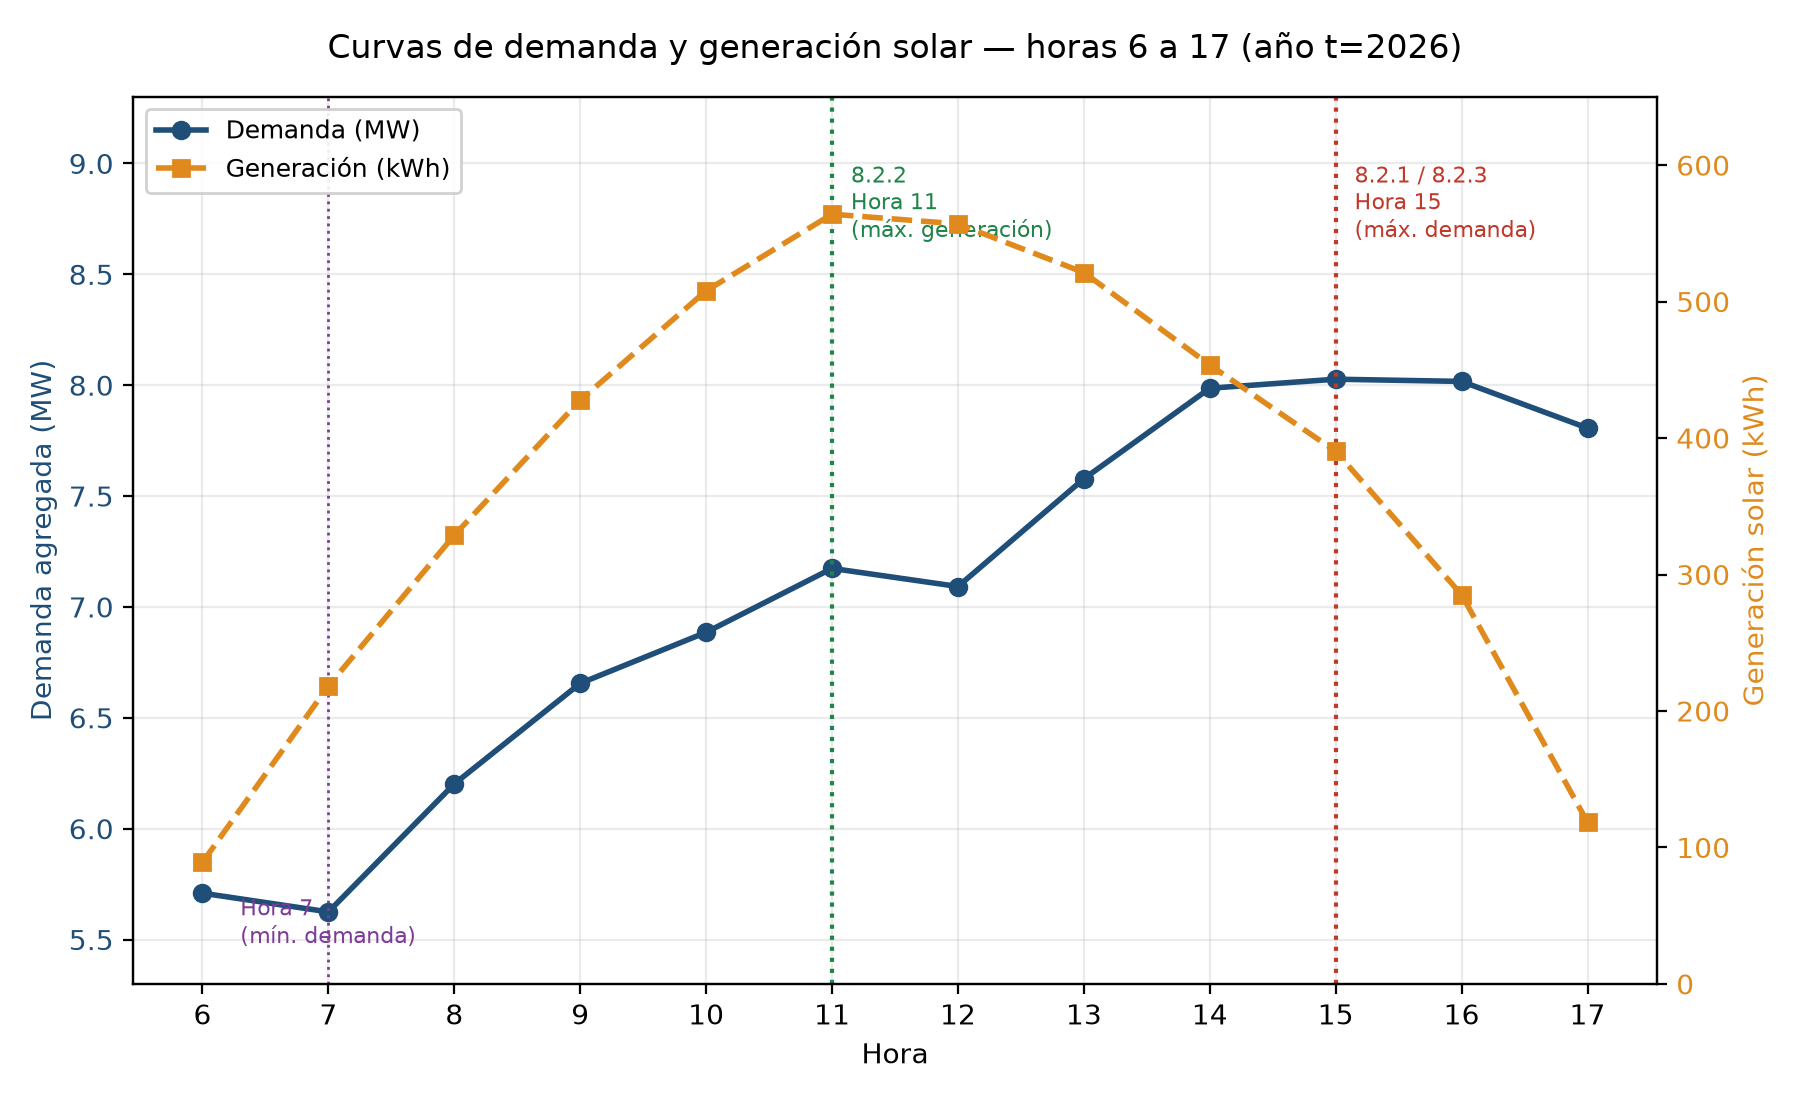
\includegraphics[width=0.95\textwidth]{curva_demanda_generacion.png}
\caption{Curvas de demanda y generaci\'on solar, horas 6-17 (a\~no $t=2026$), con los escenarios 8.2.1/8.2.2/8.2.3 identificados}
\label{fig:demanda-generacion}
\end{figure}

Cruzando \texttt{inputs/Parametros\_Demanda.xlsx} (demanda agregada de las 8 cargas del \'area de influencia) con la Tabla 16 de la memoria de c\'alculo (generaci\'on solar m\'axima por hora, Secci\'on~\ref{sec:parametros}):

\begin{table}[H]
\centering
\caption{Identificaci\'on de escenarios 8.2 con datos del proyecto}
\begin{tabular}{lccc}
\toprule
Escenario & Hora & Demanda total (MW) & Generaci\'on (kWh) \\
\midrule
8.2.1 Carga pura & 15 & 8.027 (m\'axima 6-17) & 0 (forzada) \\
8.2.2 Momento de m\'axima diferencia & \textbf{11} & 7.174 (demanda real en esa hora) & 564.05 (m\'axima) \\
8.2.3 M\'axima demanda y m\'axima generaci\'on & 15 & 8.027 (m\'axima) & 390.29 (en esa hora) \\
\bottomrule
\end{tabular}
\end{table}

\textbf{Criterio adoptado (confirmado con el interesado):} la demanda m\'inima (hora 7) y la generaci\'on m\'axima (hora 11) no coincid\'ian en la misma hora en los datos disponibles; se opt\'o por usar la \textbf{hora 11} (m\'axima generaci\'on solar real) con su demanda real asociada, por ser el caso m\'as cr\'itico de inyecci\'on de potencia (mayor riesgo de sobretensi\'on / flujo inverso en el punto de conexi\'on) -- criterio m\'as conservador para el interesado en conectarse.
\pendiente{Queda por evaluar si la demanda relevante deber\'ia ser \'unicamente la del circuito 15344 (m\'as cercana al punto de conexi\'on) en vez de la agregada de las 8 cargas del \'area de influencia.}

\subsection{Perfiles de tensi\'on y nivel de carga (flujo de carga)}
\label{sec:flujo-carga}
% 8.3
Resultados de \texttt{Flujo\_carga.py}: tensiones (p.u.\ y kV), \'angulo, cargabilidad de l\'ineas y transformadores, p\'erdidas activas/reactivas -- condici\'on normal (N), para las 12 horas simuladas (6-17).

\textbf{Sobre la condici\'on N-1 (contingencia sencilla):} \textbf{no se realiza}, justificado t\'ecnicamente: la red de la zona de influencia es \textbf{radial pura} (SE Puerto Boyac\'a $\to$ P1 $\to$ P2 $\to$ \ldots $\to$ P6, sin anillos ni alimentaci\'on de respaldo -- ver Figura~\ref{fig:demanda-generacion} y el diagrama unifilar). Un an\'alisis N-1 tiene sentido en redes malladas o con respaldo, donde perder un elemento redistribuye el flujo por caminos alternos (lo que puede generar sobrecargas en otros elementos -- eso es lo que N-1 busca detectar). En una topolog\'ia radial, perder cualquier l\'inea o el transformador \'unicamente \textbf{desenerg\'iza todo lo que est\'a aguas abajo} de esa falla -- no hay redistribuci\'on de flujo que evaluar, por lo que el an\'alisis N-1 no aporta informaci\'on adicional en este caso.

\textbf{Sobre el a\~no $t+x=2028$:} \texttt{Flujo\_carga.py} incluye la constante \texttt{ESCALA\_DEMANDA}, que multiplica toda la demanda de \texttt{Parametros\_Demanda.xlsx} (a\~no $t=2026$) por el incremento del \textbf{1.04\,\%} indicado por EBSA (Secci\'on~\ref{sec:parametros-t}) para proyectar el a\~no $t+x$. Se debe correr el script dos veces: una con \texttt{ESCALA\_DEMANDA=1.0} (a\~no $t$, resultado en \texttt{Resultados\_Flujo\_Carga\_2026.xlsx}) y otra con \texttt{ESCALA\_DEMANDA=1.0104} (a\~no $t+x$, \texttt{Resultados\_Flujo\_Carga\_2028.xlsx}). \textbf{No se necesita} una corrida separada de \texttt{Cortocircuito.py} para $t+x$: con el m\'etodo IEC 60909/VDE 0102 usado (\texttt{ildfinit=False}), el resultado de cortocircuito no depende del nivel de demanda.

\pendiente{Ejecutar ambas corridas de \texttt{Flujo\_carga.py} (a\~no $t$ y $t+x$) e insertar aqu\'i las tablas de perfiles de tensi\'on/cargabilidad filtradas a los escenarios de la Secci\'on~\ref{sec:escenarios}.}

\begin{table}[H]
\centering
\caption{Perfiles de tensi\'on -- Escenario [PENDIENTE], a\~no $t$}
\begin{tabular}{lccc}
\toprule
Barra & $U$ (p.u.) & $U$ (kV) & \'Angulo ($^\circ$) \\
\midrule
\multicolumn{4}{c}{\pendiente{completar desde Resultados\_Flujo\_Carga\_2026.xlsx}} \\
\bottomrule
\end{tabular}
\end{table}

\subsection{Contribuci\'on a la corriente de cortocircuito}
\label{sec:cortocircuito}
% 8.4
Resultados de \texttt{Cortocircuito.py}: $I_{kss}$ (kA) en todas las barras del sistema, fallas trif\'asica, bif\'asica y monof\'asica a tierra, con y sin el proyecto conectado (\texttt{CasoBase} vs.\ Network Variation del GD), para los escenarios 8.2.2 y 8.2.3.

\textbf{Correcci\'on aplicada y CONFIRMADA (2026-09-18):} el generador solar mostraba $I_{kss}=0$ en todas las fallas por falta de configuraci\'on del aporte a cortocircuito del objeto \texttt{ElmPvsys} (pesta\~na Short-Circuit VDE/IEC). Se configur\'o, por cada uno de los 3 inversores:
\begin{itemize}
    \item $I_k''{}_{3PF} = 238.2$\,A (ficha Huawei, ``Max. Output Current'' -- coincide con $\approx1.1\times I_n$).
    \item $I_k''{}_{2PF} = I_k''{}_{1PF} = 0$\,A (justificado por componentes sim\'etricas, $Z_2\approx\infty$ ya configurado).
    \item Corriente m\'axima de estado estable = 238.2\,A.
\end{itemize}
\textbf{Resultado tras volver a correr \texttt{Cortocircuito.py}}: el generador ahora muestra $I_{kss}=0.7146$\,kA en su propia barra (Puerto Boyaca 800\,V, falla trif\'asica) -- coincide casi exactamente con el valor esperado ($3\times238.2\,\text{A}=714.6\,\text{A}$). La correcci\'on qued\'o validada.

Adem\'as, en la misma corrida se agregaron a la red base los dos generadores existentes GD1 y GD2 (Secci\'on~\ref{sec:parametros}), configurados con ``No Short-Circuit Contribution'' -- se verific\'o que su aporte efectivamente aparece en 0 en las dem\'as barras, consistente con esa configuraci\'on.

\pendiente{Llenar la tabla de abajo con los valores de \texttt{Resultados\_Cortocircuito.xlsx} (barra por barra, \texttt{CasoBase} vs.\ con proyecto) y contrastar contra los 10\,kA de capacidad de corte.}

\begin{table}[H]
\centering
\caption{Icc en barras de AT/MT -- con y sin proyecto}
\begin{tabular}{lccc}
\toprule
Barra & $I_{kss}$ sin proyecto (kA) & $I_{kss}$ con proyecto (kA) & Capacidad de corte (kA) \\
\midrule
\multicolumn{4}{c}{\pendiente{completar Icc con y sin proyecto desde Resultados\_Cortocircuito.xlsx (Capacidad de corte = \textbf{10\,kA} para todas las barras de la SE, ya confirmada)}} \\
\bottomrule
\end{tabular}
\end{table}

\subsection{An\'alisis para evitar el funcionamiento en isla}
% 8.5
Se debe verificar:
\[
\left(\sum_{i=1}^{N} P_{max\,g_i}\right) + P_{g\,nuevo} \; \geq \; P_{min\,dem}
\]
\parcial{Falta el c\'alculo num\'erico con $P_{min\,dem}$ hist\'orica del circuito 15344 (se puede tomar de \texttt{Parametros\_Demanda.xlsx}, aunque esa demanda es agregada de 8 cargas -- ver misma observaci\'on que en la Secci\'on~\ref{sec:escenarios}).

\textbf{Mecanismo anti-isla (ya documentado):} el inversor Huawei SUN2000-330KTL-H1 incorpora un esquema de protecci\'on anti-isla certificado seg\'un IEC 62116 (procedimiento de ensayo de las medidas de prevenci\'on del funcionamiento en isla) e IEC 61727, avalado mediante el \textbf{Certificado de Conformidad No.\ CN-PV-220287}, expedido por los laboratorios acreditados de Intertek (ver memoria de c\'alculo, Secci\'on de cumplimiento normativo). El inversor tambi\'en cumple IEEE 1547 y el alcance de UL 1741 / IEC 62109. Queda pendiente \'unicamente la certificaci\'on en la etapa de pruebas de conexi\'on, conforme al Acuerdo 1522 de 2022.}

\subsection{An\'alisis de p\'erdidas}
% 8.6
Se eval\'ua el nivel de p\'erdidas activas y reactivas de \textbf{todos los elementos del sistema} (l\'ineas y transformadores), comparando el caso \textbf{con generador} y \textbf{sin generador} (\texttt{CasoBase} vs.\ Network Variation del GD), para a\~nos $t$ y $t+x$.
\parcial{Los datos de p\'erdidas por elemento ya los calcula \texttt{Flujo\_carga.py} (columnas \texttt{P\_perdidas\_MW} / \texttt{Q\_perdidas\_Mvar}, hojas \texttt{Lineas} y \texttt{Transformadores\_2Devanados}); falta consolidar la comparaci\'on \texttt{CasoBase} vs.\ caso con GD (suma de p\'erdidas de todo el sistema, por hora) en una tabla resumen, para ambos a\~nos.}

\subsection{An\'alisis de estabilidad}
% 8.7 -- No aplica
No aplica: el proyecto se conecta en Nivel de Tensi\'on II (13.2\,kV); el an\'alisis de estabilidad (8.7 de CREG 174) solo es exigido para conexiones en Nivel de Tensi\'on IV.

\subsection{Evaluaci\'on econ\'omica}
% 8.8 -- condicional
Condicional: solo aplica si los an\'alisis de las Secciones 5.3/5.4 identifican incumplimientos t\'ecnicos (sobrecargas, sobre/subtensiones). \pendiente{Definir aplicabilidad una vez cerrados los resultados.}

% ============================================================================
\section{Conclusiones}
\label{sec:conclusiones}
\pendiente{Redactar al cierre del estudio.}

% ============================================================================
\appendix
\section{Comprobaci\'on de coordinaci\'on de protecciones en cabecera del circuito 15344 (EACP simplificado)}
\label{sec:eacp}
% CREG 174, numeral 9.2 / Acuerdo CNO 2121 de 2026

El Acuerdo del Consejo Nacional de Operaci\'on (CNO) 2121 de 2026 (que actualiza y sustituye a los acuerdos 2087/1862/1749/\ldots, ``Requisitos de Protecciones para la conexi\'on de Sistemas de Generaci\'on en el SIN'') exige la elaboraci\'on de un Estudio de Ajuste y Coordinaci\'on de Protecciones (EACP) a partir de 0.1\,MW, por lo que este proyecto (990\,kW) aplica. Un EACP completo cubre todas las funciones de protecci\'on de la planta (27/59/50/51/50N/51N/59N/ROCOF, anti-isla, etc.) en todos los niveles de tensi\'on involucrados.

Lo que se presenta en esta secci\'on es de alcance m\'as acotado y corresponde a lo que efectivamente puede verse afectado por la conexi\'on de este proyecto: una \textbf{comprobaci\'on} de si el ajuste de protecci\'on \emph{ya existente y en operaci\'on} en la cabecera del circuito 15344 (el reconectador de la S/E Puerto Boyac\'a) sigue coordinando correctamente una vez se agrega el aporte de falla del proyecto. Las protecciones propias de la planta (a nivel de inversor y de tablero de baja tensi\'on) est\'an definidas por el fabricante y certificadas de f\'abrica (ver Secci\'on~\ref{sec:isla}, certificaci\'on anti-isla Intertek CN-PV-220287); no son objeto de ajuste por parte del promotor y por eso no se repiten aqu\'i.

Esta comprobaci\'on es una \textbf{metodolog\'ia programada}, implementada en \texttt{scripts/Coordinacion\_Protecciones.py}: a partir de los resultados de cortocircuito ya calculados y validados en la Secci\'on~\ref{sec:cortocircuito} (\texttt{Resultados\_Cortocircuito.xlsx}) y de los ajustes reales de EBSA (que no cambian de una corrida a otra), aplica de forma autom\'atica y reproducible la f\'ormula de la curva normalizada IEC~60255-151, sin c\'alculo manual ni intervenci\'on subjetiva. Si se vuelve a correr \texttt{Cortocircuito.py} (por ejemplo, tras incorporar GD1/GD2 o cualquier cambio de topolog\'ia), basta con volver a correr este script para obtener una comprobaci\'on actualizada.

\subsection{Metodolog\'ia}

La protecci\'on de cabecera del circuito 15344 est\'a ajustada por EBSA con curva \textbf{IEC Normal Inverse} (IEC~60255-151), tanto para la funci\'on de fase (51) como para la de neutro/tierra (51N), cada una con su umbral instant\'aneo asociado (50 y 50N respectivamente). El tiempo de disparo de la funci\'on temporizada se calcula como:

\begin{equation}
t(I) = \text{Dial} \times \dfrac{k}{\left(\dfrac{I}{I_{pickup}}\right)^{\alpha} - 1}, \qquad I > I_{pickup}
\label{eq:iec-ni}
\end{equation}

con $k = 0.14$ y $\alpha = 0.02$ (constantes de la norma para esta familia de curva, no calibrables). Si la corriente de falla supera el umbral instant\'aneo (50 o 50N), el rele no espera la curva temporizada: opera en un tiempo definido muy corto ($\approx 0.03$\,s, t\'ipico de un reconectador).

Para cada tipo de falla se eval\'ua la corriente de PowerFactory en la Ecuaci\'on~\ref{eq:iec-ni} usando la funci\'on correspondiente (trif\'asica $\rightarrow$ 51/50 de fase; monof\'asica $\rightarrow$ 51N/50N de neutro), en dos escenarios: \texttt{CasoBase} (sin proyecto) y con la Network Variation del proyecto activa (con proyecto). Si ambos escenarios caen en la \textbf{misma zona de operaci\'on} (temporizada o instant\'anea) con el \textbf{mismo tiempo de disparo}, se concluye que el aporte de falla del proyecto no altera la coordinaci\'on ya aprobada.

\subsection{Datos de entrada}

\textbf{Ajuste real de la protecci\'on de cabecera 15344} (\texttt{DOC\_REF\_EST\_1787069892338.pdf}, p\'ag.\,4 -- ``Curva ajustada en la protecci\'on del circuito y reconectador''; ya en \texttt{Parametros\_Proyecto.xlsx}, fila \texttt{Condiciones\_operativas}):

\begin{center}
\begin{tabular}{|l|c|c|c|}
\hline
\textbf{Funci\'on} & \textbf{Curva} & \textbf{Pickup} & \textbf{Dial / Instant\'aneo} \\ \hline
51 (fase, temporizada) & IEC Normal Inverse & 240\,A & Dial = 0.1 \\ \hline
50 (fase, instant\'aneo) & -- & 1500\,A & $t \approx 0.03$\,s \\ \hline
51N (neutro, temporizada) & IEC Normal Inverse & 60\,A & Dial = 0.1 \\ \hline
50N (neutro, instant\'aneo) & -- & 300\,A & $t \approx 0.03$\,s \\ \hline
\end{tabular}
\end{center}

Tiempo de recierre r\'apido del reconectador: 2\,s.

\textbf{Corriente de cortocircuito en la barra de cabecera} (P1\,15344, primer punto del circuito aguas abajo del reconectador), de \texttt{Resultados\_Cortocircuito.xlsx}:

\begin{center}
\begin{tabular}{|l|c|c|}
\hline
\textbf{Tipo de falla} & \textbf{Sin proyecto (CasoBase)} & \textbf{Con proyecto} \\ \hline
Trif\'asica & 4112\,A (4.112\,kA) & 4155\,A (4.155\,kA) \\ \hline
Monof\'asica & 4112\,A (4.112\,kA) & 4118\,A (4.118\,kA) \\ \hline
\end{tabular}
\end{center}

\subsection{Resultados}

\begin{figure}[h]
\centering
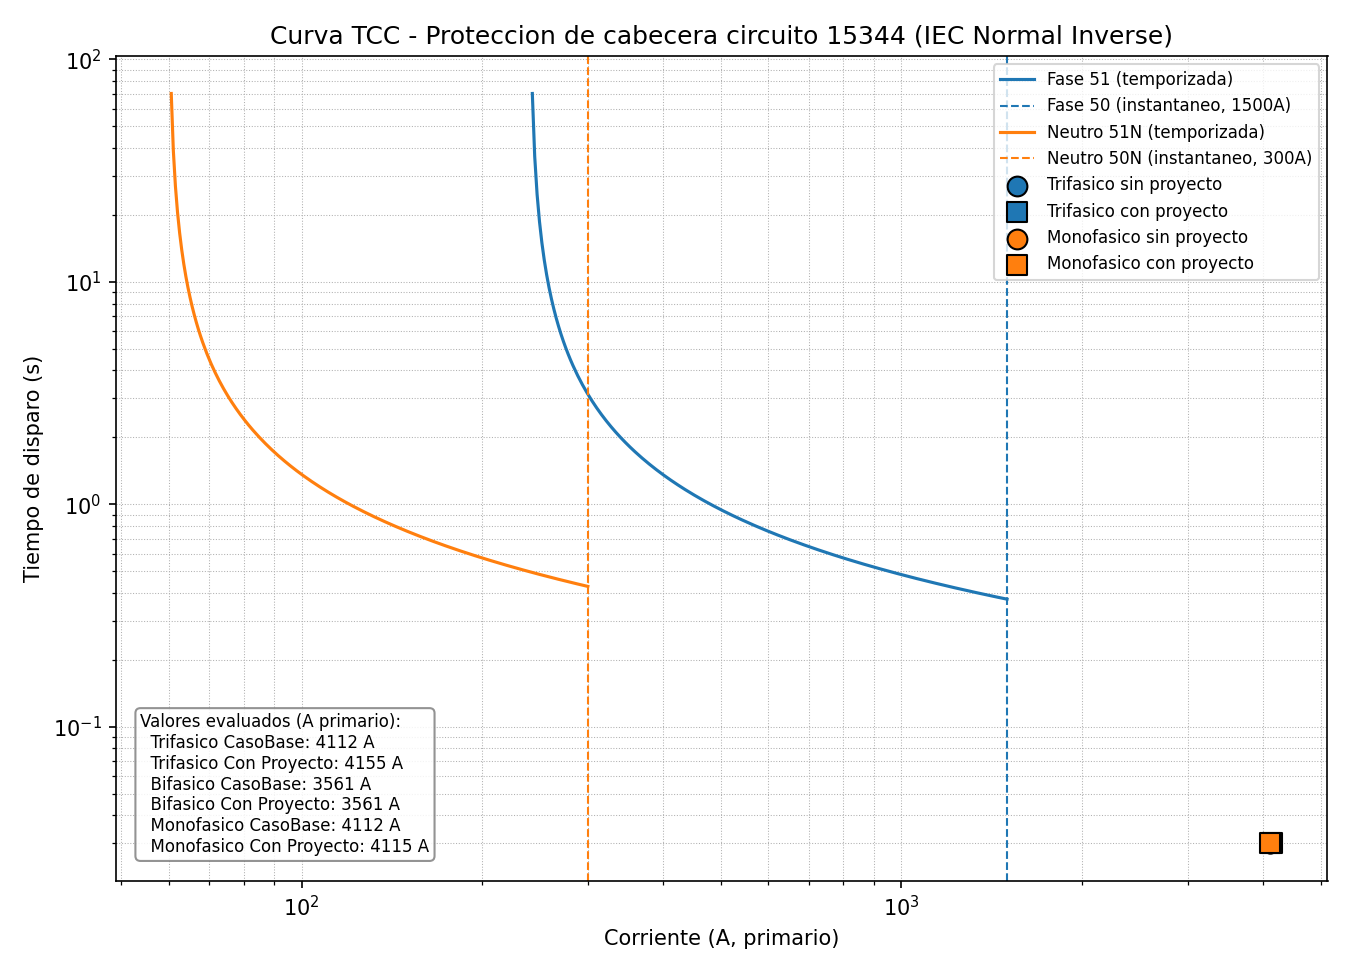
\includegraphics[width=0.85\textwidth]{Curva_TCC_Cabecera_15344.png}
\caption{Curva tiempo-corriente (TCC) de la protecci\'on de cabecera del circuito 15344 (IEC Normal Inverse), con los cuatro puntos evaluados (trif\'asico/monof\'asico, sin/con proyecto). Los cuatro puntos caen muy por encima de los umbrales instant\'aneos (1500\,A fase, 300\,A neutro), en la misma zona de operaci\'on -- por eso se ven pr\'acticamente superpuestos en la escala logar\'itmica; los valores exactos se listan en el recuadro de la gr\'afica.}
\label{fig:tcc-cabecera}
\end{figure}

En ambos tipos de falla, la corriente en cabecera (tanto sin como con el proyecto) supera ampliamente los umbrales instant\'aneos: la trif\'asica ($\sim$4.1--4.2\,kA) es $\sim$2.8 veces el umbral de fase (1500\,A), y la monof\'asica es $\sim$13.7 veces el umbral de neutro (300\,A). El aporte del proyecto desplaza la corriente en +43\,A (+1.05\,\%) para falla trif\'asica y +5.5\,A (+0.13\,\%) para falla monof\'asica -- en ambos casos, un desplazamiento marginal que no saca la falla de la zona instant\'anea ya vigente. El tiempo de disparo no cambia (0.03\,s en los cuatro casos).

\subsection{Aporte de falla del sistema de generaci\'on (insumo para malla de puesta a tierra)}

El Anexo 1 del Acuerdo CNO 2121 de 2026 liga expl\'icitamente el dise\~no de la puesta a tierra de la instalaci\'on con el sistema de protecciones propuesto, y confirma adem\'as que los sistemas de generaci\'on basados en inversores \textbf{no superan 1.1 p.u.} de su corriente nominal como aporte a la falla (limitaci\'on de la electr\'onica de potencia del inversor, no del ajuste de protecci\'on). Los valores a usar como insumo para el dise\~no de la malla de puesta a tierra del proyecto son:

\begin{center}
\begin{tabular}{|l|c|}
\hline
Aporte configurado por inversor ($Ik''_{3PF}$) & 238.2\,A \\ \hline
Corriente nominal del inversor ($330\,\text{kW} / (\sqrt{3} \times 800\,\text{V})$) & 238.2\,A \\ \hline
Aporte configurado, en p.u. de la corriente nominal & 1.00\,p.u. (dentro del l\'imite de 1.1\,p.u.) \\ \hline
Cantidad de inversores & 3 \\ \hline
\textbf{$I_{kss}$ trif\'asica validada en la barra propia del generador} & \textbf{0.7146\,kA} \\ \hline
\end{tabular}
\end{center}

El aporte se configur\'o exactamente igual a la corriente nominal del inversor (1.0\,p.u.), consistente con el comportamiento t\'ipico de un inversor limitador de corriente ante falla, y el resultado de la simulaci\'on en PowerFactory (0.7146\,kA) qued\'o validado contra el c\'alculo esperado ($3 \times 238.2\,\text{A} = 714.6\,\text{A}$, ver Secci\'on~\ref{sec:cortocircuito}).

\subsection{Conclusiones y recomendaciones}

\begin{itemize}
\item El aporte de falla del proyecto en la cabecera del circuito 15344 es marginal (+1.05\,\% trif\'asico, +0.13\,\% monof\'asico) frente al nivel de cortocircuito de la red de EBSA, y \textbf{no requiere reajuste} del reconectador de cabecera: ambos escenarios (sin y con proyecto) operan en la misma zona instant\'anea, con el mismo tiempo de disparo.
\item El l\'imite regulatorio de aporte a falla para tecnolog\'ia basada en inversores (1.1\,p.u., Anexo 1 del Acuerdo 2121) se cumple con margen: el proyecto qued\'o configurado en 1.0\,p.u.
\item Seg\'un el Anexo 1 del Acuerdo 2121, para proyectos entre 0.25\,MW y 1\,MW (este proyecto: 990\,kW) se exige en el punto de conexi\'on un interruptor con unidades de disparo, reconectador o interruptor de potencia, con capacidad de interrupci\'on acorde al nivel de cortocircuito del estudio de conexi\'on. \pendiente{Confirmar/documentar el equipo de corte en el lado de media tensi\'on (13.2\,kV) del transformador propio del proyecto -- pendiente detectado en el levantamiento de este numeral.}
\item Esta comprobaci\'on cubre \'unicamente la coordinaci\'on en cabecera del circuito. Las funciones de protecci\'on propias de la planta (inversor y tablero) ya est\'an cubiertas por la certificaci\'on de f\'abrica citada en la Secci\'on~\ref{sec:isla}.
\end{itemize}

\section{Checklist de causales de rechazo (Tabla 6, CREG 174)}
Ver \texttt{informe/Estructura\_Informe\_Conexion.xlsx}, hoja \texttt{Causales\_Rechazo}, para el detalle y estado de cada causal.

\end{document}
